\section{Simulation results and discussion}
\label{sec:simulation_result}
%Pour le papier, il n'est pas nécessaire de montrer les résultats de simulation et les résultats du modèle analytique dans tous les cas. Tu peux montrer que les 2 coïncident dans un ou 2 cas puis faire l'analyse en te basant uniquement sur les résultats du modèle. Cela permettra de présenter plus de cas sur le même graphique. Je verrais bien une analyse avec -3 dB, -1 dB, 0 dB, +1dB, +3 dB comme pas de modification de puissance. 
%Il peut être intéressant de comparer les résultats du cas IV et du cas V. 
%
%Inutile de présenter les mêmes résultats avec 2 échelles différentes. Je pense que tu peux choisir l'échelle logarithmique. Utilise tout le temps la même échelle : 10-6 à 1 semble bien (ou 10-4 à 1) . 
\subsection{Accuracy of proposed models}
To verify the accuracy of proposed analytical model, we develop a Python-based simulator. In each simulation, we define $N$ M2M devices. Each device generates a fresh packet with probability of $\alpha/N$ in each slot. The total number of packets generated by all devices during one slot approximately follows a Poisson distribution with intensity $\alpha$ if $\alpha/N$ is enough small. In case of transmission failure, a retransmission is scheduled after a random number of slots following exponential distribution with mean of $50$ slots. To calculate $95\%$ confidence interval, simulation is repeated $40$ times for each arrival intensity.

For the diversity of transmit power, we consider three strategies: \begin{inparaenum}[1)]
	\item identical transmit power level $v=1$; 
	\item incremented transmit power level with factor $v=2$;
	\item decremented transmit power level with factor $v=0.5$.
\end{inparaenum}
The maximum allowed retransmission number $K$ is set as $4$. In terms of capture effect, we confirm our analytical model under three SINR threshold: $3$dB, $0$dB, $-3$dB.  

To confirm the accuracy of analytical model, only the packet loss rate results obtained from analytical model and simulation ($95 \%$ confidence interval) are shown. Fig.~\ref{fig:ideal_ci} illustrates the comparison for the ideal system. The case of wide-band system affected by imperfect power control is shown  in Fig.~\ref{fig:ci}. Fig.~\ref{fig:ci_fading_shadowing} illustrates the results for the system that suffers Rayleigh fading and imperfect power control.
In these three figures, we observe that, the proposed analytical results coincide with that of simulation in most cases. There exists a difference between analytical and simulation result in Fig.~\ref{fig:ci}(c), when fresh packet arrival rate $\alpha$ is between $1.08$ and $1.1$. For regime of interest, from $10^{-3}$ to $10^{-1}$, the proposed models still give accurate estimation of packet loss rate.

\begin{figure*}[!ht]
	\centering
	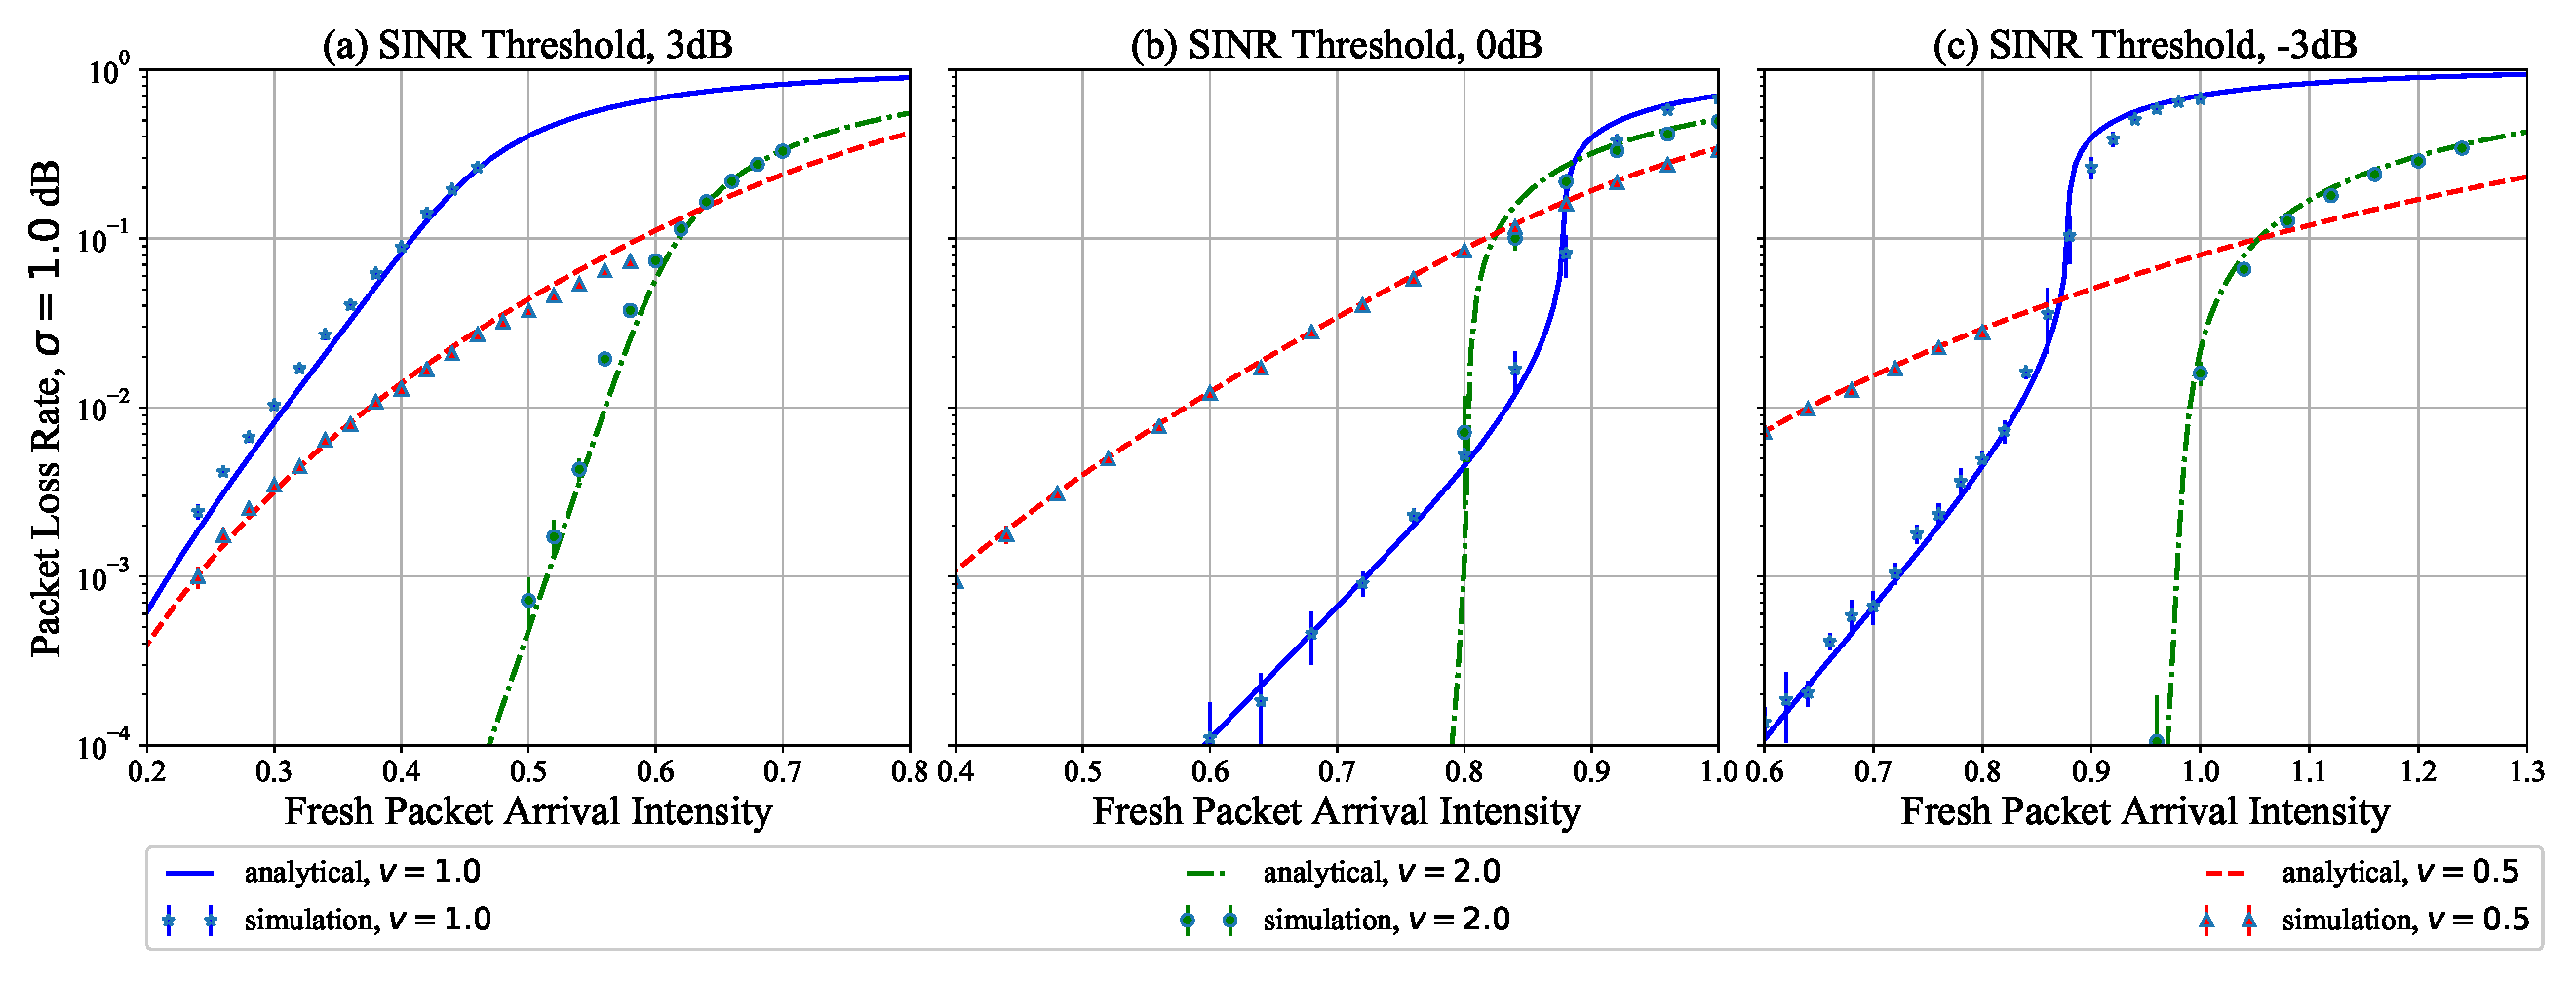
\includegraphics[width=1.0\linewidth]{Chapter4/Figures/packet_loss_rate_ci_with_ideal.eps}
	\caption{Packet loss rate of S-ALOHA under one ideal system}
	\label{fig:ideal_ci}
\end{figure*}

\begin{figure*}[!ht]
	\centering
	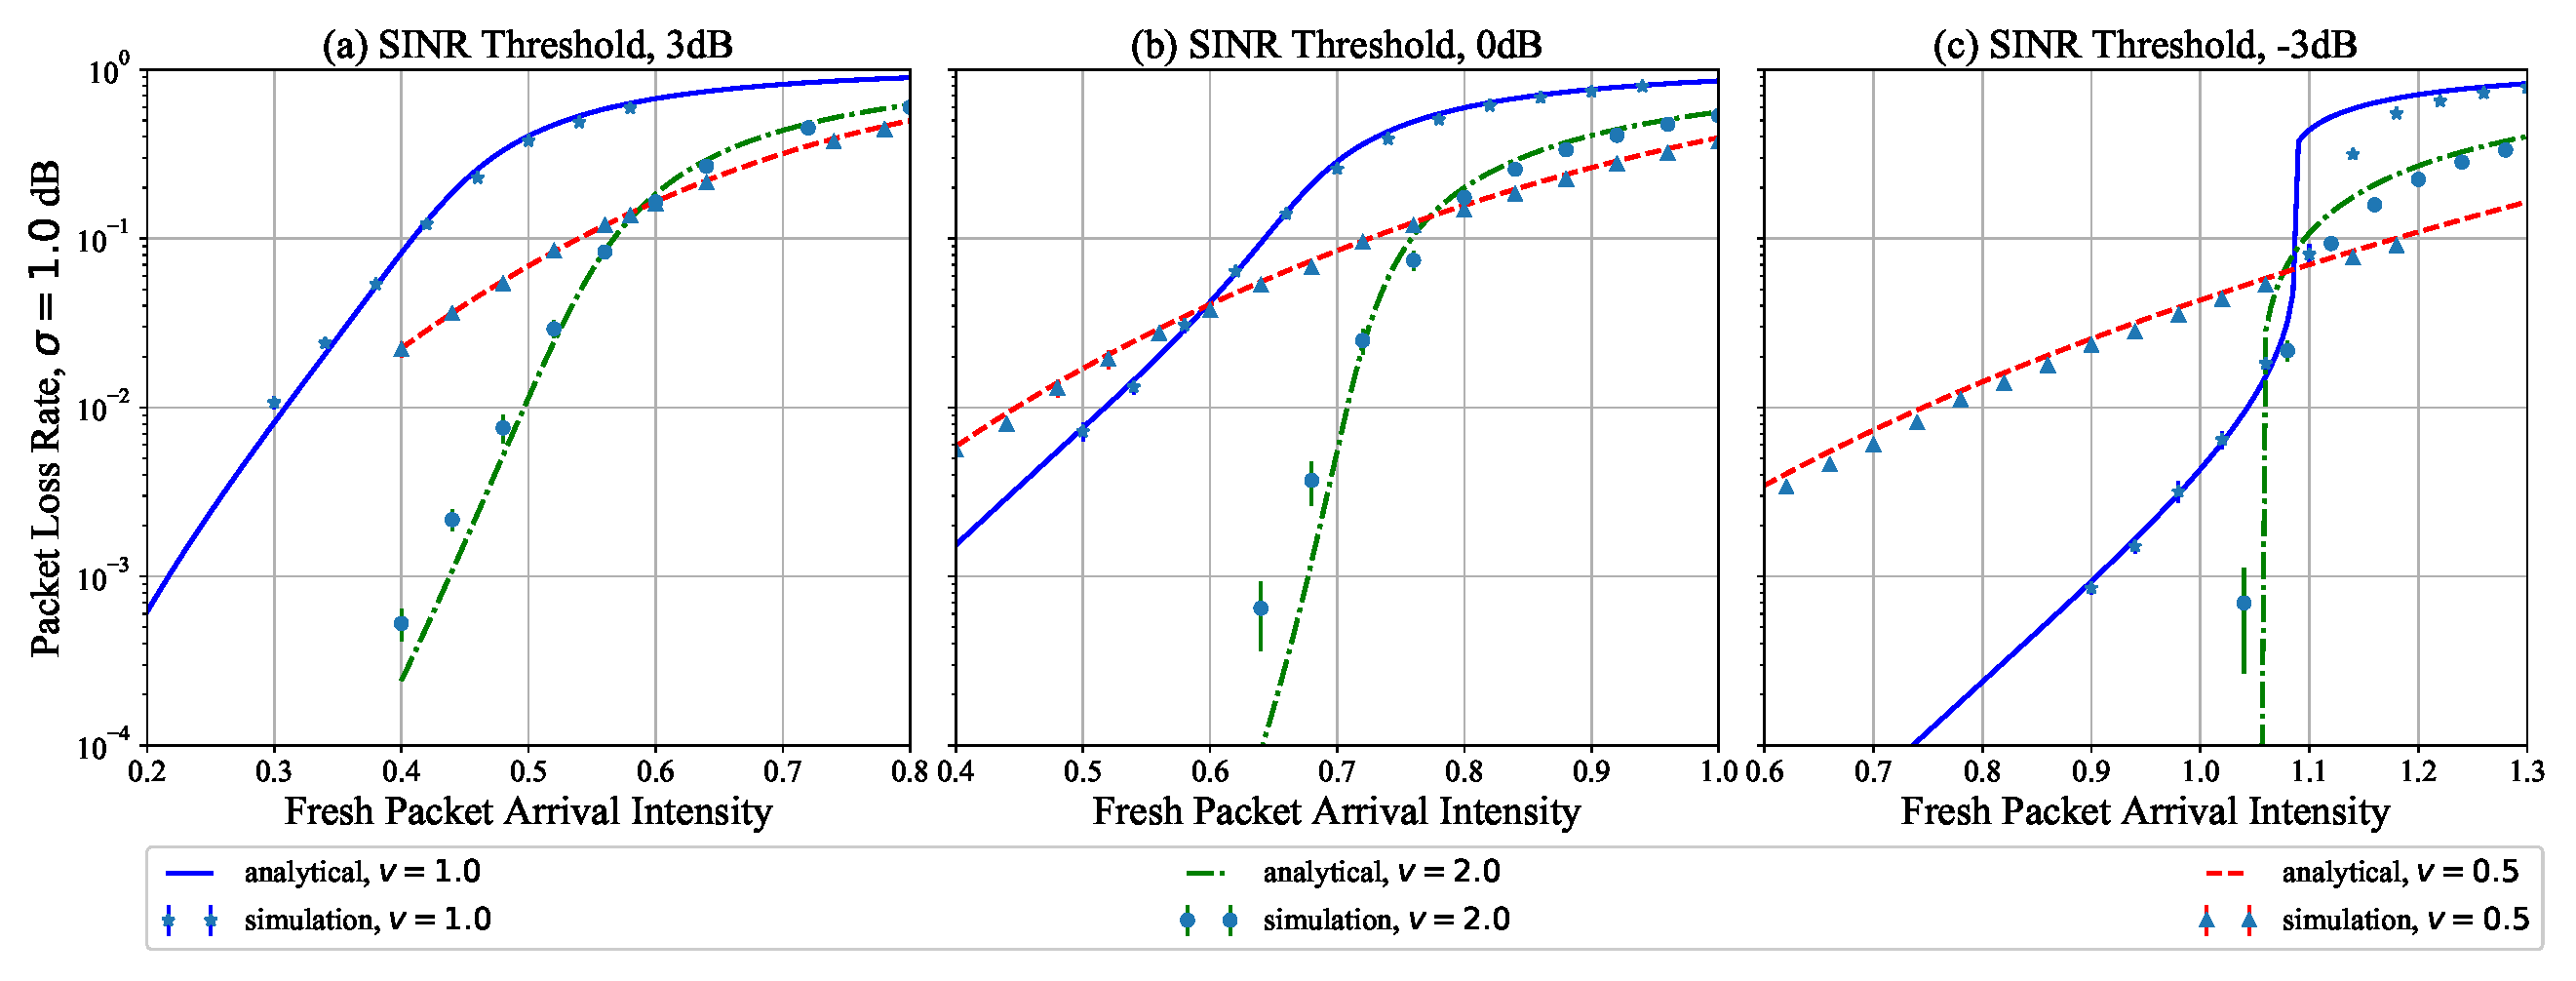
\includegraphics[width=1.0\linewidth]{Chapter4/Figures/packet_loss_rate_ci.eps}
	\caption{Packet loss rate of S-ALOHA under wide-band system. The power control error is $1$dB}
	\label{fig:ci}
\end{figure*}

\begin{figure*}[!ht]
	\centering
	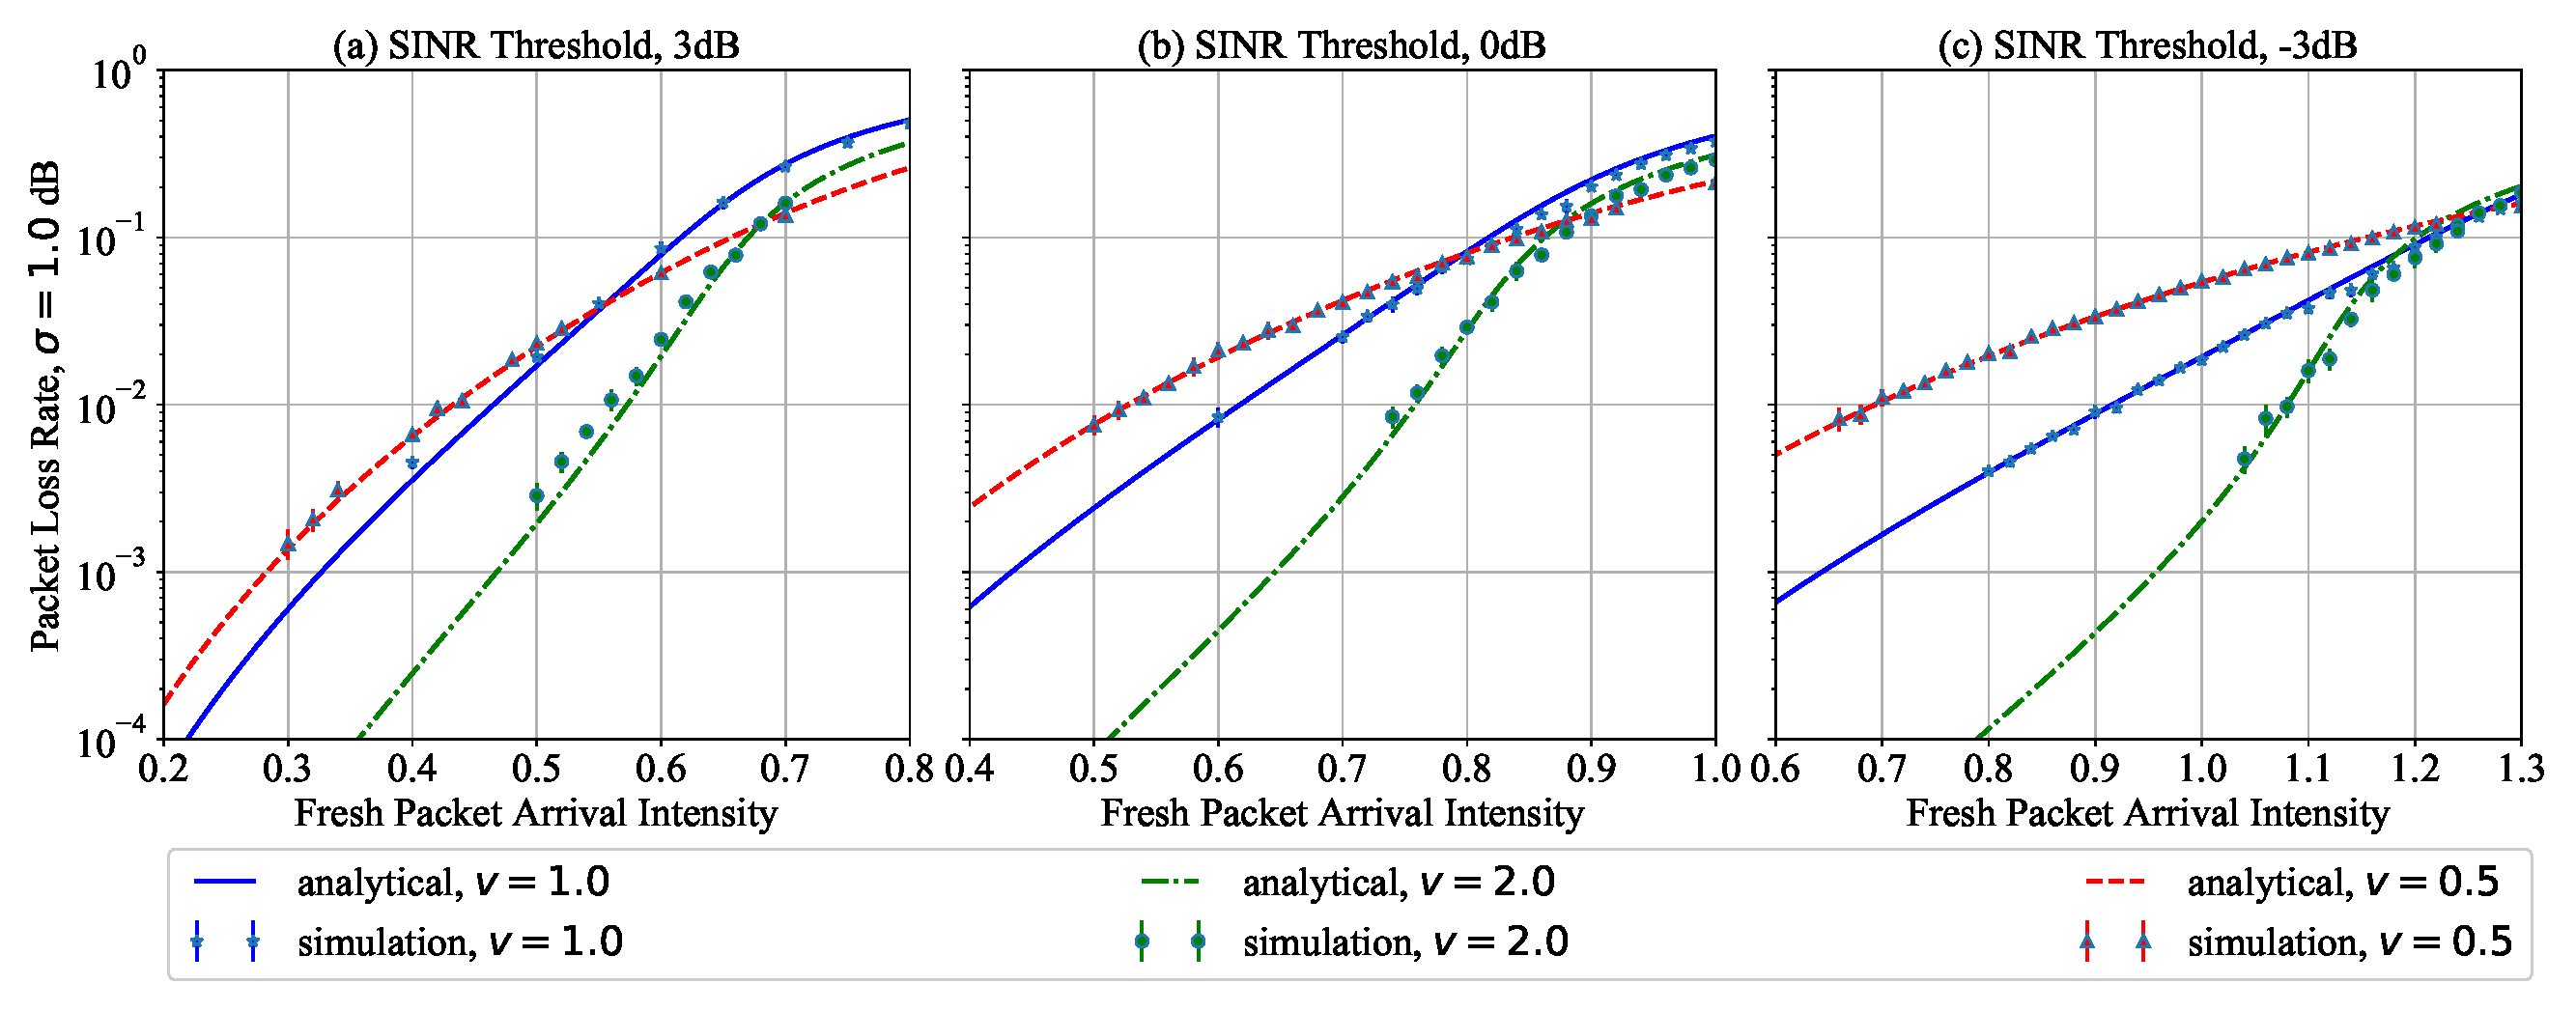
\includegraphics[width=1.0\linewidth]{Chapter4/Figures/packet_loss_rate_ci_with_fading_shadowing.eps}
	\caption{Packet loss rate of S-ALOHA in networks suffered fading and imperfect power control. The power control error is $1$dB}
	\label{fig:ci_fading_shadowing}
\end{figure*}

For a given arrival rate $\alpha$, with our proposed analytical models, the probability vector can be obtained by less than $30$ iterations, within several seconds. This means that the proposed models can be integrated into M2M network dimensioning tools box.
\subsection{Performance evaluation under different settings}

\begin{figure*}[!h]
	\centering
	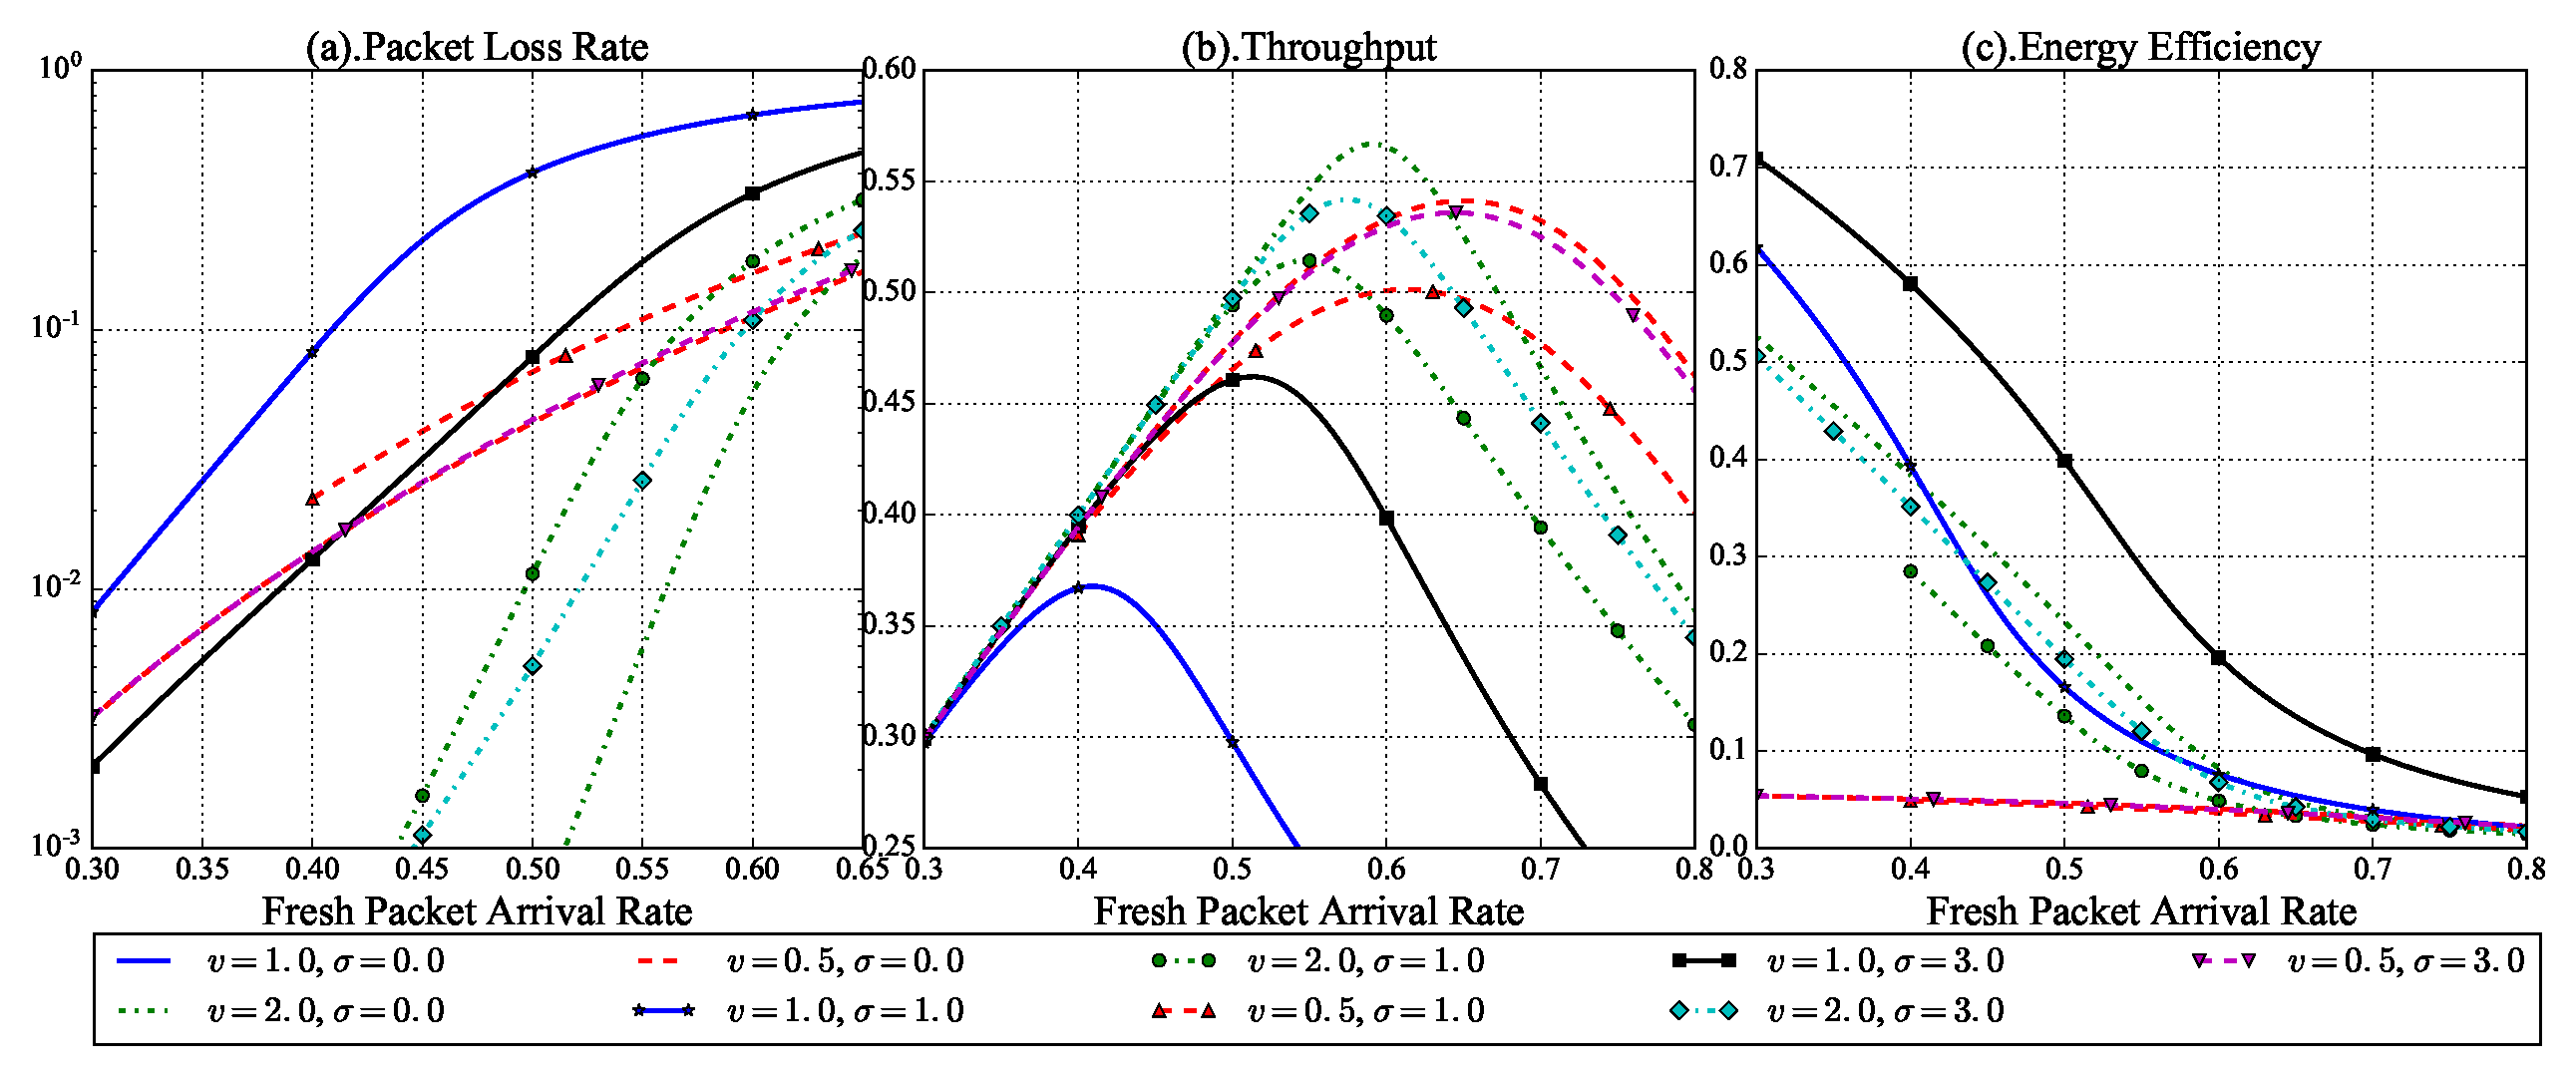
\includegraphics[width=1.0\linewidth]{Chapter4/Figures/shadowing_performance_case_3.0.eps}
	\caption{Performance comparison under SINR threshold $3$dB. Each sub-figure shows the comparison under three different power control error standard deviation $\sigma = 0, 1, 3$dB. Note that $\sigma=0.0$dB refers to the perfect power control case.}
	\label{fig:shadowing_performance}
\end{figure*}

The S-ALOHA in M2M networks is evaluated with packet loss rate, throughput, energy efficiency. Due to limitation of space, the performance of average number of transmission is not plotted in the figure. We compare the performance under power control error $0$dB (i.e., perfect power control), $1$dB, $3$dB in each figure. The case of perfect power control serves as comparison reference.

 In Fig.~\ref{fig:shadowing_performance} with SINR threshold $3$dB, we observe that the imperfect power control has positive impact if $v=1$, namely with identical transmit strategy. When power control error standard variance is $1$dB, the performance of S-ALOHA is identical with perfect power control case (the solid line with stars completely superposes with solid line). When the standard deviation of power control error is $3$dB, the S-ALOHA performance with identical transmit strategy gets improved (comparing the solid line with square and solid line with stars). In this case, power control error acts as a way to make transmit power levels more diverse and improve the performance. For other two strategies $v=2$ and $v=0.5$, the imperfect power control degrades the performance of S-ALOHA, because power control error reduces the transmit powers levels diversity introduced by factor $v$. In Fig.~\ref{fig:shadowing_performance}(c), S-ALOHA using identical transmit power outperforms than other strategies in terms of energy-efficiency. The energy-efficiency of decremental power strategy is always at low level, since this strategy requires to start with high power levels. 

%The aforementioned observations tell us that: with presence of capture effect relatively high, instead of pursuing precise power control in device side, S-ALOHA can get improved with poor power control, since the latter make the transmit power levels more diverse.
\begin{figure*}[!th]
	\centering
	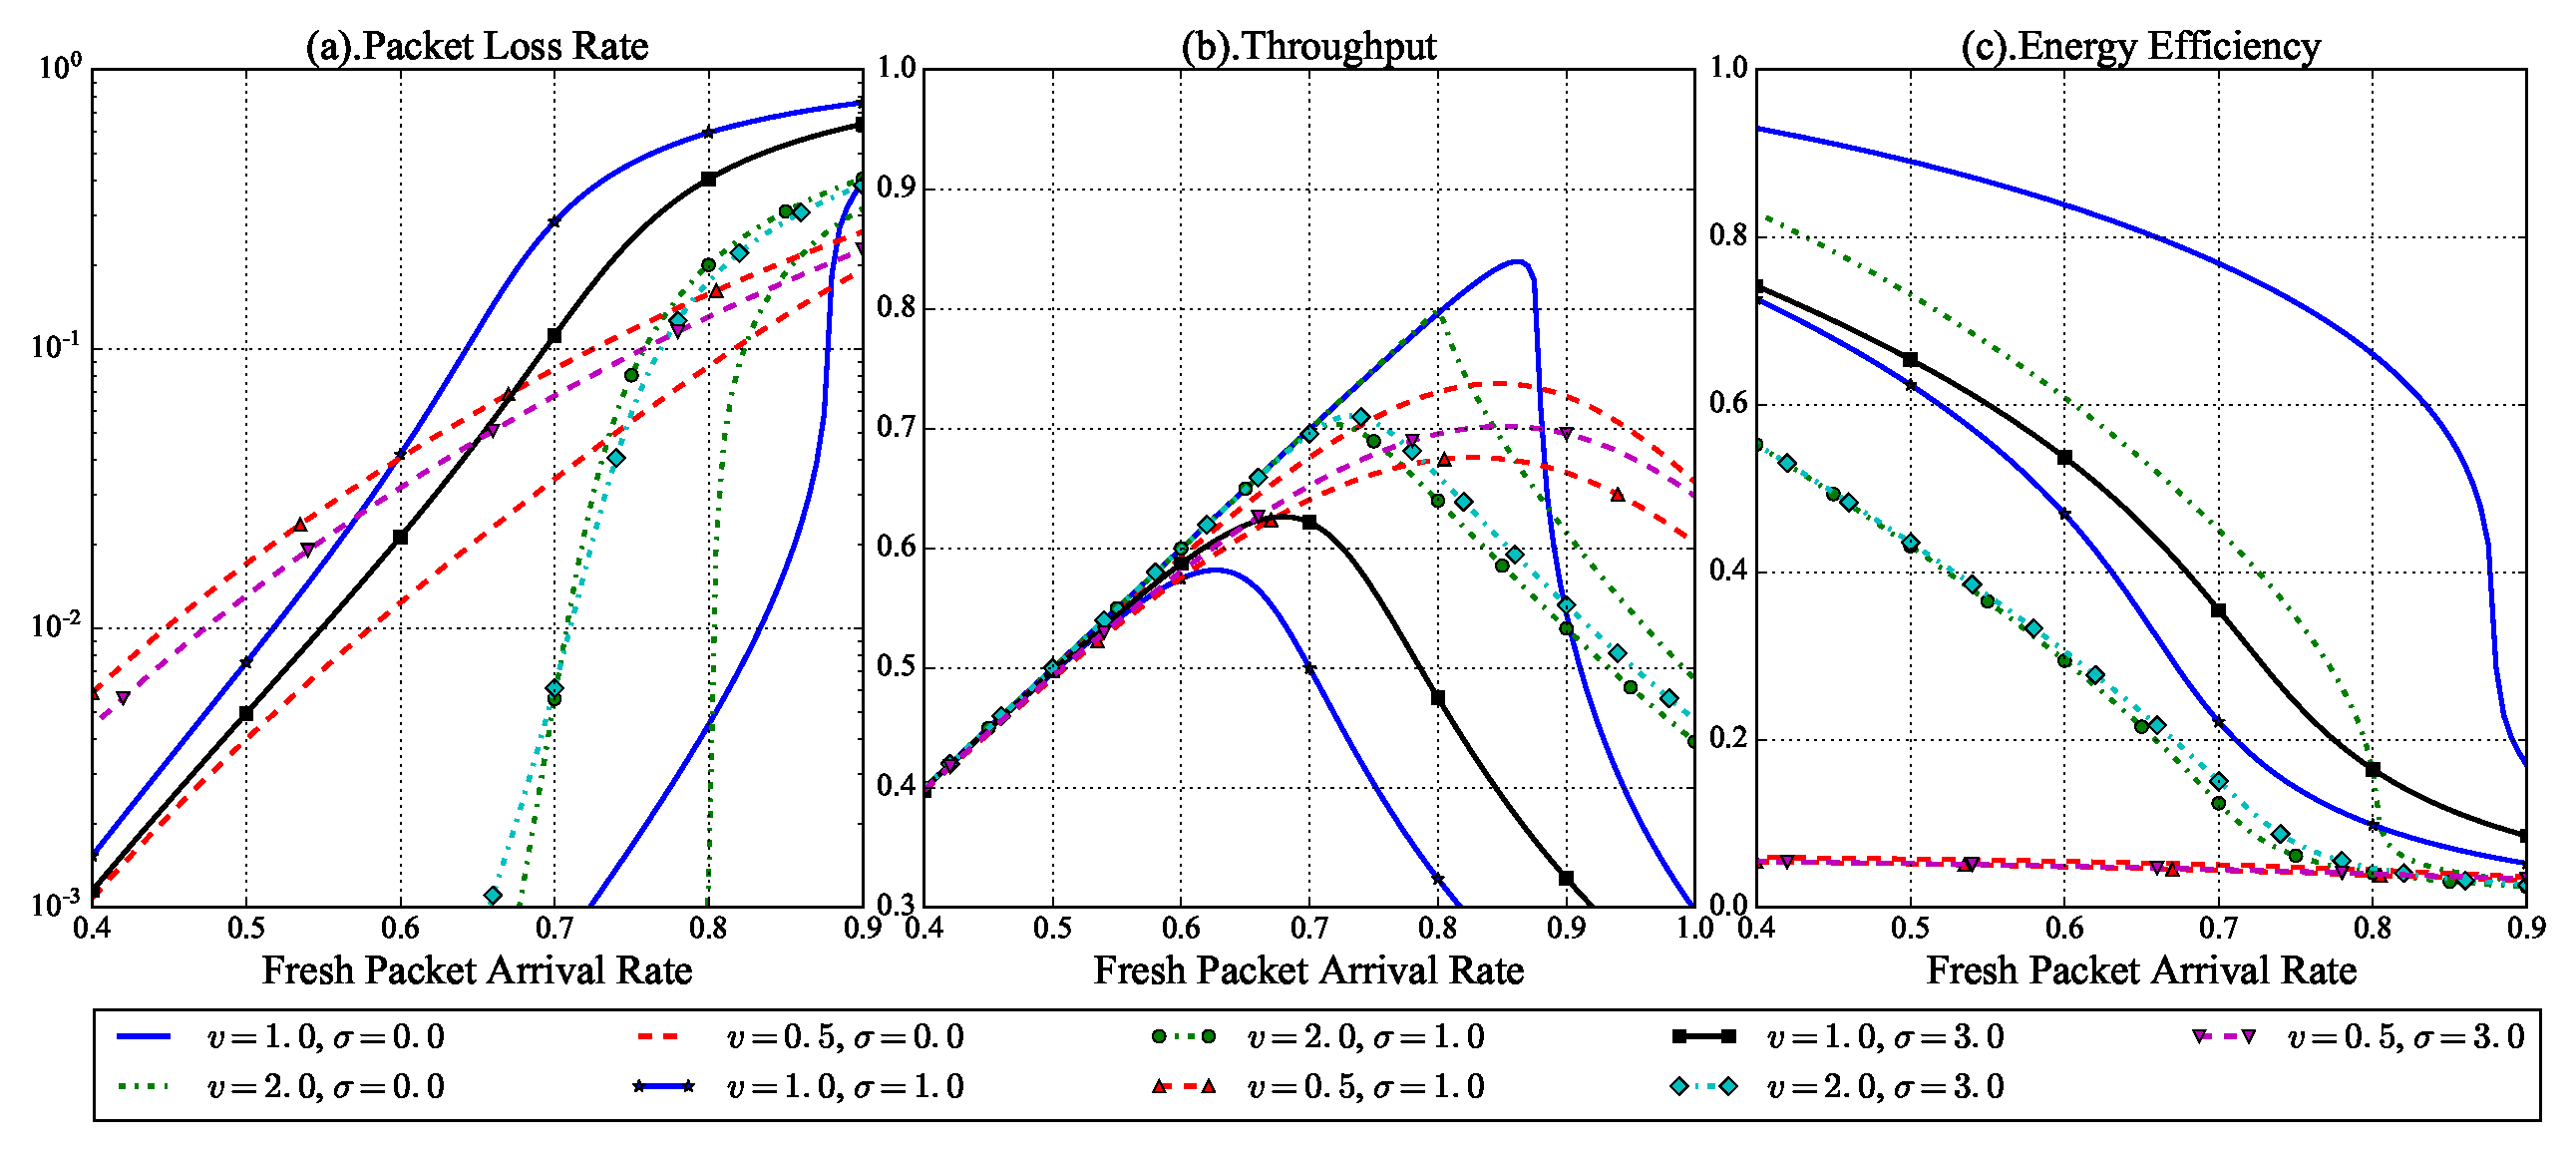
\includegraphics[width=1.0\linewidth]{Chapter4/Figures/shadowing_performance_case_0.0.eps}
	\caption{Performance comparison under SINR threshold $0$dB. Each sub-figure shows the comparison under three different power control error standard deviation $\sigma = 0, 1, 3$dB. Note that $\sigma=0.0$dB refers to the perfect power control case.}
	\label{fig:shadowing_performance_0}
\end{figure*}

Fig.~\ref{fig:shadowing_performance_0} shows the comparison result under capture ratio $0$dB. In this case, the performance of S-ALOHA gets worse due to power control error no matter which strategy is employed. For all three power strategies, the performance of power control error $3$dB is better than that of $1$dB, since serious power control error makes the transmit power more diverse. With such a capture ratio, the best choice of diversity strategy depends on the privileged performance metric. For example, for a network preferring energy-efficiency to throughout, S-ALOHA with identical power strategy is recommended option. Otherwise, S-ALOHA with incremental power strategy is better. 

\begin{figure*}[!th]
	\centering
	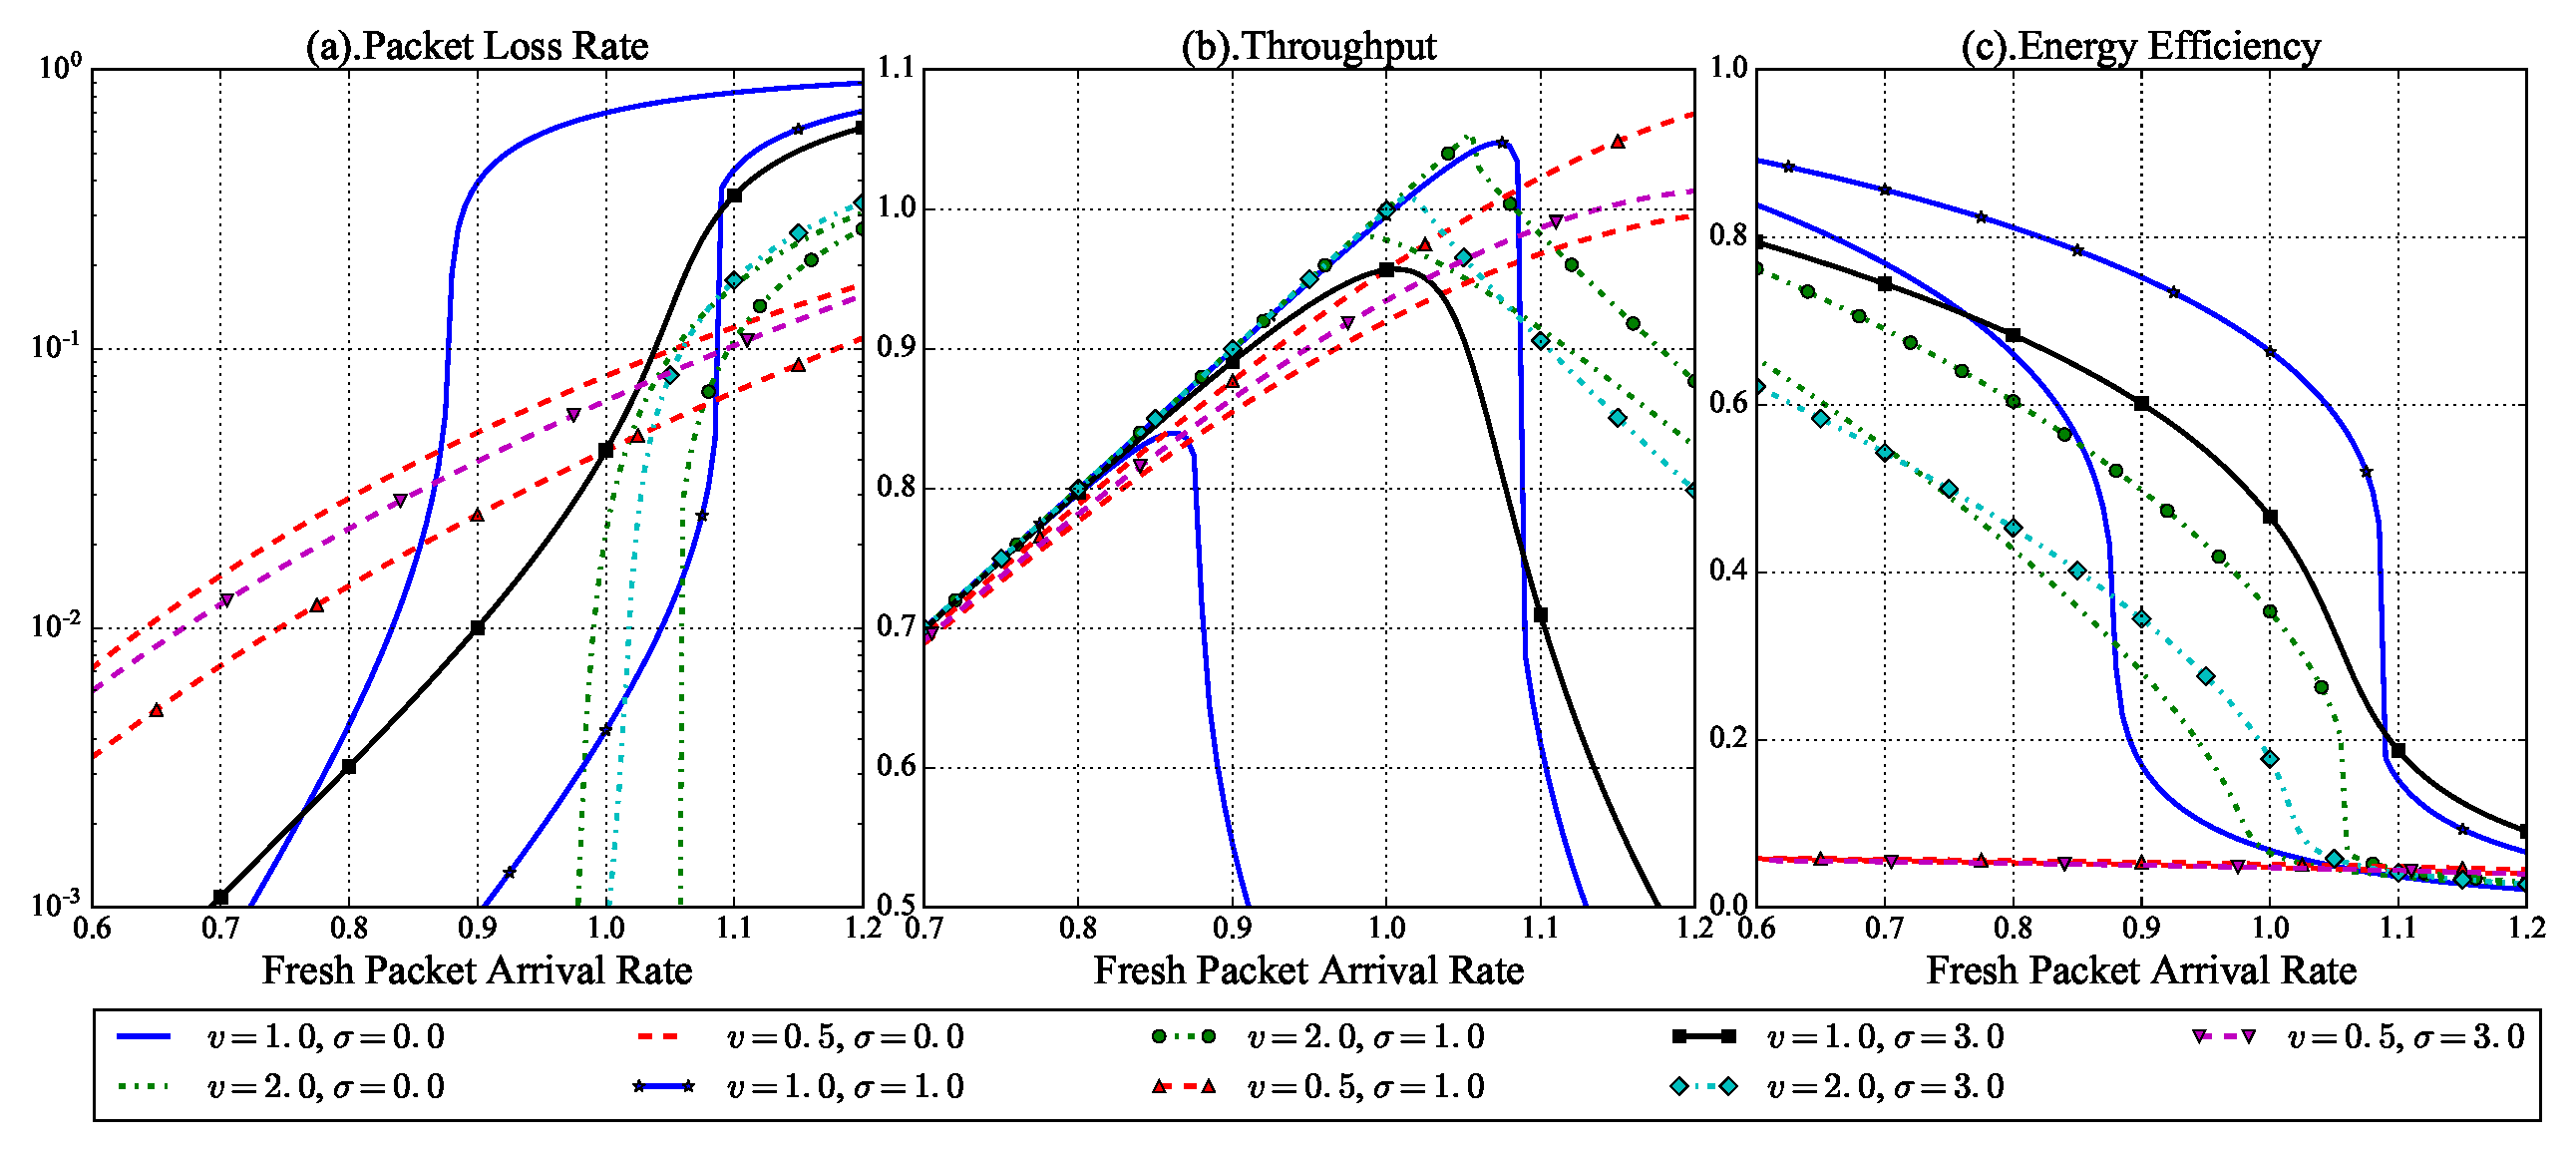
\includegraphics[width=1.0\linewidth]{Chapter4/Figures/shadowing_performance_case_-3.0.eps}
	\caption{Performance comparison under SINR threshold $-3$dB. Each sub-figure shows the comparison under three different power control error standard deviation $\sigma = 0, 1, 3$dB. Note that $\sigma=0.0$dB refers to the perfect power control case.}
	\label{fig:shadowing_performance_-3}
\end{figure*}
Fig.~\ref{fig:shadowing_performance_-3} where SINR threshold is $-3$dB refers to a spectrum-spreading system. In this case, the power control error always has a positive impact on S-ALOHA. S-ALOHA achieves a better performance when the power control is more precise. In addition, the choice of transmit power diversity depends on fresh packet arrival rate. For example, when the standard deviation of power control error is $1$dB, if networks based on S-ALOHA are still unsaturated (i.e, with fresh arrival rate less than $1.1$), identical strategy is better than others. With arrival rate greater than $1.1$, the throughput  is sharply reduced. The decremental strategy starts to be a better choice.
 
%Precisely, it has an obvious impact when power increment factor is less than its standard error.


%\begin{figure}[!th]
%	\centering
%	\includegraphics[width=1.0\linewidth]{Figures/logarithme_shadowing_case1.eps}
%	\caption{The Packet Loss Rate evolution with respect to the fresh packet arrival intensity. The SINR threshold for a successful packet transmission is $3$ dB. The effects of power increment, power decrement and no power change are all shown in the same figure.}
%	\label{fig:shadowing_case1}
%\end{figure}
%
%\begin{figure}[!th]
%	\centering
%	\includegraphics[width=1.0\linewidth]{Figures/logarithme_shadowing_case2.eps}
%	\caption{The Packet Loss Rate evolution with respect to the fresh packet arrival intensity. The SINR threshold for a successful packet transmission is $0$ dB. The effects of power increment, power decrement and no power change are all shown in the same figure.}
%	\label{fig:shadowing_case2}
%\end{figure}
%
%\begin{figure}[!th]
%	\centering
%	\includegraphics[width=1.0\linewidth]{Figures/logarithme_shadowing_case3.eps}
%	\caption{The Packet Loss Rate evolution with respect to the fresh packet arrival intensity. The SINR threshold for a successful packet transmission is $-3$ dB. The effects of power increment, power decrement and no power change are all shown in the same figure.}
%	\label{fig:shadowing_case3}
%\end{figure}


%\subsection{Fading and imperfect power control}
%\subsubsection{Case1: 3dB}
%From Fig.~\ref{fig:fading_case1}, we observe that when the predefined SINR threshold is set as $3$dB, for the case power increment, power decrement and no power change, the simulation and analytical results are well coherent. Also, we find that for the packet loss rate range of interest (i.e., from $10^{-2}$ to $10^{-1}$), it is the power increment case which always has the best performance (i.e., support higher packet arrival intensity with same packet loss loss rate)
%\begin{figure}[!th]
%	\centering
%	\includegraphics[width=\linewidth]{Figures/logarithme_fading_case1.eps}
%	\caption{The Packet Loss Rate evolution with respect to the fresh packet arrival intensity. The SINR threshold for a successful packet transmission is $3$ dB. The effects of power increment, power decrement and no power change are all shown in the same figure.}
%	\label{fig:fading_case1}
%\end{figure}
%
%\subsubsection{Case2: 0dB}
%From Fig.~\ref{fig:fading_case2}, we observe that the simulation result is well superposed with analytical result. Also, we find that for the packet loss rate range of interest (i.e., from $10^{-2}$ to $10^{-1}$), it is the power increment case which always has the best performance (i.e., support higher packet arrival intensity with same packet loss loss rate). However, around packet loss rate as $10^{-1}$, the performance gain of power increment case (dashdot line) is small compared with case of power decrement (dashed line).
%\begin{figure}
%	\centering
%	\includegraphics[width=\linewidth]{Figures/logarithme_fading_case2}
%	\caption{The Packet Loss Rate evolution with respect to the fresh packet arrival intensity. The SINR threshold for a successful packet transmission is $0$ dB.}
%	\label{fig:fading_case2}
%\end{figure}
%
%\subsubsection{Case3: -3dB}
%From Fig.~\ref{fig:fading_case3}, we observe that the simulation result is well superposed with analytical result. Also, we find that for the packet loss rate range of interest (i.e., from $10^{-2}$ to $10^{-1}$), it is the power increment case which always has the best performance (i.e., support higher packet arrival intensity with same packet loss loss rate). However, around packet loss rate as $10^{-1}$, the performance gain of power increment case (dashdot line) is small compared with case of identical power (continuous line).
%\begin{figure}
%	\centering
%	\includegraphics[width=\linewidth]{Figures/logarithme_fading_case3}
%	\caption{The Packet Loss Rate evolution with respect to the fresh packet arrival intensity. The SINR threshold for a successful packet transmission is $-3$ dB.}
%	\label{fig:fading_case3}
%\end{figure}
